\section{Relational Queries in CouchDB}
CouchDB uses MapReduce as a deterministic means of producing indices using parallel processing; MapReduce is implemented in terms of index requirements rather than as a means of performing relational operations on datasets. As such, performing relational operations on datasets using CouchDB's implementation of MapReduce is impossible and instead requires architecture-wide considerations. This is in contrast to RDBMSs where relational operations are isolated to the data retrieval layer and require much less thought into entity modeling, software stack architectures, etc. as a result.

But in the context of this project it is shown that CouchDB data can be modeled relationally, and relational operations can be performed on such data in the context of CouchDB. To do this requires the following considerations:

\begin{enumerate}
    \item ETL processes incorporate operations that would more generally be used in the data-retrieval layer in RDBMSs - i.e. projections, selections (include selections via joins)
    \item MapReduce is used as a means of normalizing entity representation, performing aggregations and sorting entity representations according to join-keys
    \item Joins can be performed quite easily and efficiently on sorted indices
\end{enumerate}

Although indices may be time-consuming to calculate initially, scanning b+trees is very efficient and so data retrieval from CouchDB is fast once indexed. And since indices are updated incrementally, joins performed via index scans are also very efficient. This in itself is an advantage offered by CouchDB when used in a relational context. However, working with relational data is clearly more difficult in CouchDB than in any RDBMS and most other NoSQL alternatives as well.

% TODO
discuss why it's beneficial to use this means of entity modelling instead of aggregations in a nosql database

\section{Software Performance}
Performance metrics of the different components of the system are recorded and are shown in Table \ref{tbl-metadata} showing running time of nETL tasks, a summary of the data processed by nETL, CouchDB indexing times, and database/index storage footprints.

\begin{table}[H]
    \begin{threeparttable}
        \textbf{Table \ref{tbl-metadata}}\par\medskip\par\medskip
        \caption[Software performance analysis]{Running time analysis of \textit{nETL} tasks and CouchDB MapReduce indexing}
        \label{tbl-metadata}
        \begin{tabularx}{\textwidth}{>{\hsize=1.6\hsize}X>{\hsize=0.8\hsize}Y>{\hsize=0.8\hsize}Y>{\hsize=0.8\hsize}Y}
            \toprule
            \mC{c}{}                                                & \mC{c}{Adms}                      & \mC{c}{Adms/Grds}                  & \mC{c}{Adms/Grds/Evts}               \\
            \midrule
            Admissions lines extracted                              & 12 219                            & 12 219                             & 12 219                               \\
            Admissions lines loaded                                 & 1 381                             & 1 381                              & 595                                  \\
            Admissions task time (sec)                              & 1.588\tnote{\textsuperscript{1a}} & 2.712\tnote{\textsuperscript{1b}}  & 4.935\tnote{\textsuperscript{1c}}    \\
            \midrule
            Grades lines extracted                                  &                                   & 513 872                            & 513 872                              \\
            Grades lines loaded                                     &                                   & 1 891                              & 738                                  \\
            Grades task time (sec)                                  &                                   & 50.993\tnote{\textsuperscript{2a}} & 97.532\tnote{\textsuperscript{2b}}   \\
            \midrule
            Events lines extracted                                  &                                   &                                    & 44 420 508                           \\
            Events lines loaded                                     &                                   &                                    & 661 555                              \\
            Events task time (sec)                                  &                                   &                                    & 3 875.932\tnote{\textsuperscript{3}} \\
            \midrule
            Data footprint (MB)                                     & $<$ 1                             & $<$ 2                              & 169.5                                \\
            Index calculation time (sec)\tnote{\textsuperscript{*}} & 0.533\tnote{\textsuperscript{4a}} & 1.092\tnote{\textsuperscript{4b}}  & 140.763\tnote{\textsuperscript{4c}}  \\
            \bottomrule
        \end{tabularx}
        \scriptsize
        \begin{tablenotes}
            \item[\textsuperscript{*}]CouchDB views are calculated per shard. By default a database contains 8 shards (even in single node mode). The log file shows start and end times of view calculations for each shard, the time is taken as time the first shard starts indexing, to the time the last shard stops indexing
            \item[\textsuperscript{1a}]$1.502, 1.745, 1.518$
            \item[\textsuperscript{1b}]$3.045, 2.787, 2.305$
            \item[\textsuperscript{1c}]$5.313, 3.548, 5.782, 5.095$
            \item[\textsuperscript{2a}]$52.899, 51.399, 48.681$
            \item[\textsuperscript{2b}]$94.353, 92.902, 100.134, 102.738$
            \item[\textsuperscript{3}]$3989.82, 3942.93, 3695.046$
            \item[\textsuperscript{4a}]$0.519, 0.472, 0.607$
            \item[\textsuperscript{4b}]$0.988, 1.347, 0.941$
            \item[\textsuperscript{4c}]$141.25, 142.709, 138.331$
        \end{tablenotes}
    \end{threeparttable}
\end{table}

\section{Student Profiling}
An important property of any benchmarking method is the variance of the datasets from which these benchmarks are drawn. Small variance will magnify small discrepancies between students and as such does not provide a useful means of assessing students for university admission. Obviously the higher the degree of correlation between benchmarking methods and course grades the better.

An ideal benchmark has a high degree of correlation with a large variance. Obviously benchmarking methods should be applicable to as large a group of students as possible (for example, although additional mathematics may be a good means of assessing incoming student's abilities, it is useless since so few students take this subject in matric).

Statistical output as calculated during index retrieval is shown in:

\begin{itemize}
    \item Table \ref{tbl-variance-benchmarks}: Variance of benchmarks datasets
    \item Table \ref{tbl-correlation-grades}: Correlation between final CSC1015F results with different benchmark datasets
    \item Table \ref{tbl-correlation-events}: How change in classrank between final CSC1015F and different benchmark datasets correlates with general Sakai usage
\end{itemize}

\begin{table}[H]
    \begin{threeparttable}
        \textbf{Table \ref{tbl-variance-benchmarks}}\par\medskip\par\medskip
        \caption{Variance and Std. Deviation of different possible metrics for benchmarking students during admissions}
        \label{tbl-variance-benchmarks}
        \begin{tabularx}{\textwidth}{>{\hsize=1.6\hsize}X>{\hsize=0.7\hsize}Y>{\hsize=0.7\hsize}Y}
            \toprule
            \mC{c}{Benchmark}                      & \mC{c}{$(\sigma_{\overline{x}})^{2}$} & \mC{c}{$\sigma_{\overline{x}}$} \\
            \midrule
            Gr12 Eng \%                            & 56                                    & 7.5                             \\
            Gr12 Sci \%                            & 101.5                                 & 10.1                            \\
            Gr12 Mth \%                            & 68.1                                  & 8.3                             \\
            NBT AL \%                              & 91.2                                  & 9.6                             \\
            NBT QL \%                              & 176.5                                 & 13.3                            \\
            NBT Mth \%                             & 193.8                                 & 13.9                            \\
            Avg Gr12 \%                            & 52.5                                  & 7.2                             \\
            Avg Gr12 \% (Dbl Mth)                  & 53.3                                  & 7.3                             \\
            Avg Gr12 \% (Dbl Mth \& Sci)           & 59                                    & 7.7                             \\
            Avg NBT \%                             & 102.3                                 & 10.1                            \\
            Avg NBT \% (Dbl AL)                    & 89.7                                  & 9.5                             \\
            Avg NBT \% (Dbl QL)                    & 113.8                                 & 10.7                            \\
            Avg NBT \% (Dbl Mth)                   & 113                                   & 10.6                            \\
            Avg NBT \% (Dbl AL/QL)                 & 99.6                                  & 10                              \\
            Avg NBT \% (Dbl AL/Mth)                & 92.3                                  & 9.6                             \\
            Avg NBT \% (Dbl QL/Mth)                & 117.1                                 & 10.8                            \\
            Avg Gr12 \& NBT                        & 59.4                                  & 7.7                             \\
            Avg Gr12 \& NBT (Dbl Gr12 Mth)         & 55.3                                  & 7.4                             \\
            Avg Gr12 \& NBT (Dbl Gr12 Mth  \& Sci) & 59.1                                  & 7.7                             \\
            \bottomrule
        \end{tabularx}
    \end{threeparttable}
\end{table}
\begin{table}[H]
    \begin{threeparttable}
        \textbf{Table \ref{tbl-correlation-grades}}\par\medskip\par\medskip
        \caption{Correlation between different benchmarking methods and CSC1015F grades}
        \label{tbl-correlation-grades}
        \begin{tabularx}{\textwidth}{>{\hsize=1.3\hsize}X>{\hsize=0.7\hsize}Y}
            \toprule
            \mC{c}{Benchmark}                     & \mC{c}{$r$} \\
            \midrule
            Gr12 Eng \%                           & 0.287       \\
            Gr12 Sci \%                           & 0.465       \\
            Gr12 Mth \%                           & 0.447       \\
            NBT AL \%                             & 0.368       \\
            NBT QL \%                             & 0.533       \\
            NBT Mth \%                            & 0.510       \\
            Avg Gr12 \%                           & 0.485       \\
            Avg Gr12 \% (Dbl Mth)                 & 0.487       \\
            Avg Gr12 \% (Dbl Mth \& Sci)          & 0.493       \\
            Avg NBT \%                            & 0.583       \\
            Avg NBT \% (Dbl AL)                   & 0.559       \\
            Avg NBT \% (Dbl QL)                   & 0.580       \\
            Avg NBT \% (Dbl Mth)                  & 0.583       \\
            Avg NBT \% (Dbl AL/QL)                & 0.567       \\
            Avg NBT \% (Dbl AL/Mth)               & 0.570       \\
            Avg NBT \% (Dbl QL/Mth)               & 0.589       \\
            Avg Gr12 \& NBT                       & 0.610       \\
            Avg Gr12 \& NBT (Dbl Gr12 Mth)        & 0.587       \\
            Avg Gr12 \& NBT (Dbl Gr12 Mth \& Sci) & 0.578       \\
            \bottomrule
        \end{tabularx}
    \end{threeparttable}
\end{table}
\begin{table}[H]
    \begin{threeparttable}
        \textbf{Table \ref{tbl-correlation-events}}\par\medskip\par\medskip
        \caption{Correlation Sakai presence and (course class rank - benchmark class rank)}
        \label{tbl-correlation-events}
        \begin{tabularx}{\textwidth}{>{\hsize=1.3\hsize}X>{\hsize=0.7\hsize}Y}
            \toprule
            \mC{c}{Benchmark}                     & \mC{c}{$r$} \\
            \midrule
            Gr12 Eng \%                           & 0.007       \\
            Gr12 Sci \%                           & -0.091      \\
            Gr12 Mth \%                           & -0.038      \\
            NBT AL \%                             & 0.144       \\
            NBT QL \%                             & 0.166       \\
            NBT Mth \%                            & 0.017       \\
            Avg Gr12 \%                           & -0.073      \\
            Avg Gr12 \% (Dbl Mth)                 & -0.070      \\
            Avg Gr12 \% (Dbl Mth \& Sci)          & -0.076      \\
            Avg NBT \%                            & 0.119       \\
            Avg NBT \% (Dbl AL)                   & 0.128       \\
            Avg NBT \% (Dbl QL)                   & 0.138       \\
            Avg NBT \% (Dbl Mth)                  & 0.087       \\
            Avg NBT \% (Dbl AL/QL)                & 0.141       \\
            Avg NBT \% (Dbl AL/Mth)               & 0.120       \\
            Avg NBT \% (Dbl QL/Mth)               & 0.111       \\
            Avg Gr12 \& NBT                       & 0.016       \\
            Avg Gr12 \& NBT (Dbl Gr12 Mth)        & -0.012      \\
            Avg Gr12 \& NBT (Dbl Gr12 Mth \& Sci) & -0.048      \\
            \bottomrule
        \end{tabularx}
    \end{threeparttable}
\end{table}

\subsection{Variance of Different Student Profiling Methods}
Only admissions data with values for all Gr12 grades (except math literacy and additional maths) and NBT results were considered resulting with a sample size of \mintinline{text}{n = 908} students over 3 years.

\subsection{Correlating CSC1015F Grades With Admissions Data}
Correlation between the Grades and various combinations of the Benchmarks data shows that compared to Gr12 results, the NBT scores correlate better with CSC1015F performance. The highest correlation between benchmarking and CSC1015F course results occurs when the NBT scores are averaged, with either the NBT QL or NBT Mth (or both) scores double weighted; such a correlation is 0.50, which is considered a moderate correlation.

\subsection{Correlating Sakai Usage With Academic performance}
Because the event data doesn't contain a foreign key to the grade entities, it is only possible assess the count of presence events for all sites in relation to the CSC1015F site. This isn't particularly useful, and perhaps is the main reason that no correlation is found. However this analysis is useful in demonstrating how such a correlation can be performed using CouchDB making such an analysis somewhat worthwhile.

Taking the NBT QL benchmark as an example (which has a comparatively high correlation with course grades compared to other benchmarks), the \( \delta \) class rank of benchmark score vs grade score is plotted against presence event count of each student in \ref{fig-delta-rank} for a visual feel of how the correlation analysis plots. The correlation between course grades (for CSC1015F) and LMS usage is relatively insignificant according to these results.

\begin{figure}[H]
    \centering
    % \begin{mdframed}
    % \centering
    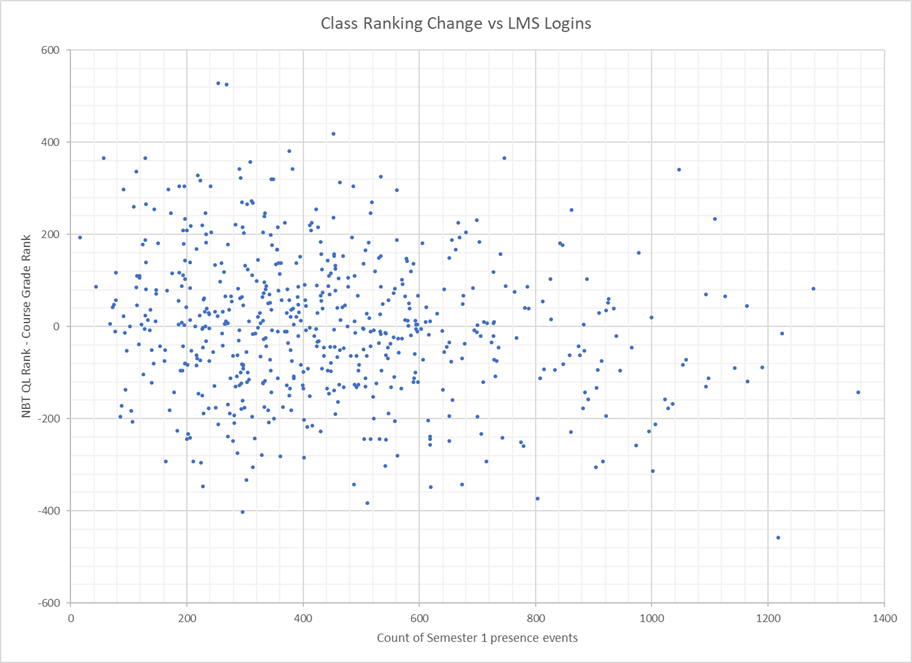
\includegraphics[scale=0.6]{./resources/figures/delta-class-rank.png}
    % \end{mdframed}
    \caption[\( \delta \) class rank vs LMS Logins]{\textbf{Figure \ref{fig-delta-rank}: \( \delta \) class rank vs LMS Logins.} An example of the correlation between \( \delta \) NBT QL ranking scores/course grades compared to LMS usage.}
    \label{fig-delta-rank}
\end{figure}